\documentclass[english]{ltugboat}
\usepackage{babel}
\usepackage[T1]{fontenc}
\usepackage{multicol}
\usepackage{calc}
\usepackage[simplified]{pgf-umlcd}
\usetikzlibrary{calc}
\usepackage{graphicx}
\usepackage{microtype}
\usepackage[hidelinks,pdfa]{hyperref}
\usepackage{listings}
% For colored variants see:
%   https://github.com/Xerdi/texmf-packaging
%\usepackage{lstlangjson}
%\usepackage{lstlangyaml}
\usepackage{subcaption}
\usepackage{ulem}
\usepackage{wasysym}
\usepackage{dirtree}
\title{Specifying and Populating Documents in YAML with lua-placeholders in LaTeX}

% repeat info for each author; comment out items that don't apply.
\author{Erik Nijenhuis}
\address{Frans Halsstraat 38\\ Leeuwarden, 8932 JC \\ The Netherlands}
\netaddress{erik (at) xerdi dot com}
\personalURL{https://github.com/MacLotsen}
%\ORCID{0}
% To receive a physical copy of the TUGboat issue, please include the
% mailing address we should use, as a comment if you prefer it not be printed.

% Tikz setup
\renewcommand{\umltextcolor}{black}
\renewcommand{\umlfillcolor}{white}
\renewcommand{\umldrawcolor}{black}

\def\pkg#1{\texttt{#1}}

\lstset{
    columns=fullflexible,
    basicstyle=\ttfamily,
    keywordstyle={\upshape},
    keywordstyle=[2]{\upshape},
    commentstyle={\itshape},
    stepnumber=1,
    numbersep=5pt,
    numberstyle=\ttfamily\footnotesize\itshape,
    showspaces=false,
    showstringspaces=false,
    showtabs=false,
    tabsize=4,
    breaklines=true,
    captionpos=b,
    breakatwhitespace=false
}

% Style shorthands
\lstdefinestyle{tex}{
    language={[LaTeX]TeX}
}

\lstdefinestyle{yaml}{
    language=yaml
}

\lstdefinestyle{json}{
    language=json
}

\begin{document}
    \maketitle

    \begin{abstract}
        This article examines the implementation of the invoice template in GinVoice and explores how the invoice template can better align with the \LaTeX\ ecosystem by introducing an additional data layer in YAML using \texttt{lua-placeholders}. With the introduction of \texttt{lua-placeholders}, \LaTeX\ users have complete freedom in formatting invoice templates, and the invoice templates are directly integratable with the enhanced version of GinVoice.
    \end{abstract}

    \section*{Keywords}
    \LuaLaTeX, YAML

    \section{Introduction}
During my work as a Software Engineer, I encountered a challenge for a company that drafts agreements and terms for multiple clients.
One of the challenging aspects was keeping client data and regulatory documentation separate.
Previously, I addressed this challenge in GinVoice\cite{ginvoice} by generating additional \LaTeX\ files with Python, which were then compiled alongside the main \LaTeX\ file.
However, this time, my goal was to provide a solution from within the \LaTeX\ domain itself, rather than the application domain.
The solution I developed, now known as \pkg{lua-placeholders}\cite{lua-placeholders}, introduces a shared data layer with YAML between \LaTeX\ and application code.
The package provides an intermediary layer specifically for data through YAML files.
To demonstrate this solution, we take GinVoice as an example.
This example, a Python GTK application that generates invoices with \LaTeX, offers slightly more complexity and challenges than the legal domain has to offer.

\subsection{The Compiler -- \LuaLaTeX}
My decision to use \LuaLaTeX\ as the compiler had several reasons.
Since 2016, I have been using \LuaLaTeX, which greatly helped me with documents within computer science at the time.
Over the years, I have gained a lot of experience in compiling with \LuaLaTeX\ and see it as a suitable compiler as a developer, thanks to the ability to script in Lua, which I naturally appreciate as a programmer.

The ability to script in Lua offers several advantages.
It allows me to perform complex tasks during the compilation process, such as processing YAML files or manipulating and structuring data. Additionally, \LuaLaTeX\ supports Lua init scripts, allowing me to implement a custom compilation process with its own CLI (Command Line Interface), further simplifying and optimizing the integration process for end solutions.

\subsection{What is YAML?}
As a DevOps Engineer, I have often encountered YAML while working with tools such as Docker Compose, Travis CI, GitHub Actions, and Canonical's NetPlan (Ubuntu systems).
YAML is widely used in the DevOps world for automating and managing configurations, functioning as a structured markup language for defining configuration files and capturing infrastructural and operational aspects of software applications.

YAML has become a crucial component of modern software development and deployment due to its simple syntax and flexibility. In combination with \LaTeX, YAML provides a powerful mechanism for defining and managing structured data, which is particularly useful when integrating client data into \LaTeX\ documents. Listing~\ref{lst:example} shows an example of YAML used in conjunction with \LaTeX.

\begin{lstlisting}[language=YAML,caption={\ttfamily invoice-001.yaml},label={lst:example}]
supplier: grapefruit
client: juicing-joker
title: Grapefruit Inc. Invoice
subtitle: for fruits and stuff
currency: \$
number: 1
date: \today
...
\end{lstlisting}


    \section{Legacy Factuur}

Dit hoofdstuk richt zich op de bestaande implementatie van de factuurtemplate in GinVoice en de noodzaak om deze te upgraden naar een meer flexibele en geautomatiseerde oplossing met behulp van \pkg{lua-placeholders}.
We zullen de huidige \LaTeX-template van de factuur bekijken en identificeren welke delen ervan vervangen kunnen worden.
Daarnaast zullen we de structuur van de factuurdata analyseren en bespreken waarom bepaalde onderdelen zijn opgesplitst.
Tot slot zullen we de beperkingen van het huidige systeem bespreken en de voordelen van de overgang naar \pkg{lua-placeholders} benadrukken.
Het gebruik van \pkg{lua-placeholders} zal uitgebreider worden behandeld in het volgende hoofdstuk.
Deze verandering stelt ons in staat om een meer efficiënte en flexibele facturatieoplossing te creëren die volledig geïntegreerd is in het LaTeX-domein.

\subsection{\LaTeX-template}
Belangrijk om te weten van de huidige implementatie is dat GinVoice\cite{ginvoice} een Python script -- \texttt{generator.py} -- gebruikt om extra \TeX-bestanden te genereren.
Die \TeX-bestanden worden vervolgens in de template ingeladen met \cs{include}, zodat de benodigde macro's beschikbaar zijn.
Uiteraard zal dat niet meer het geval zijn na het introduceren van \pkg{lua-placeholders}.
Hier is de code binnen de \texttt{document} omgeving:
\lstinputlisting[name=invoice-original,language={[LaTeX]TeX},firstnumber=52,linerange={52-55},numbers=left,xleftmargin=15pt]{ginvoice/invoice-original.tex}
De eerste drie regels hebben enkel te maken met de \cs{makeheader} macro afkomstig van \texttt{invoice.cls} en in de preamble van dit bestand is er een gekleurde laag aan toegevoegd met behulp van een pakket uit KommaScript—\pkg{scrlayer-scrpage}.
De \cs{makeheader} maakt intern gebruik van de \cs{title} en \cs{subtitle} macro's, die later nog aan bod komen.
\lstinputlisting[name=invoice-original,language={[LaTeX]TeX},firstnumber=56,linerange={56-67},numbers=left,xleftmargin=15pt]{ginvoice/invoice-original.tex}
Deze bijzondere \texttt{tabular} constructie zorgt ervoor dat het adres van de klant (\cs{addressee}) samen met factuurinformatie (\cs{customerinfo}) links komt te staan en de leveranciersinformatie (\cs{supplierinfo}) rechts.
\lstinputlisting[name=invoice-original,language={[LaTeX]TeX},firstnumber=69,linerange={69-72},numbers=left,xleftmargin=15pt]{ginvoice/invoice-original.tex}
Op regel 69 zie je dat het gegenereerde \TeX-bestand verlaat wordt ingeladen.
Dit heeft typisch te maken met het calculatieproces van de kolombreedtes.
Namelijk, de pagina dimensies zijn in de preamble nog onbekend, of kunnen nog veranderen.
Een opmerkelijke functionaliteit daarentegen is de variabele kolomdefinitie, iets wat met \pkg{lua-placeholders} alsnog knap lastig kan worden.
De macro's die vervangen gaan worden zijn \cs{tablefooter} voor de eindtotalen en \cs{tablerecords} voor de factuurregels.
De andere onbekende macro's verplaatsen we van applicatieniveau naar het documentniveau.
\lstinputlisting[name=invoice-original,language={[LaTeX]TeX},firstnumber=74,linerange={74-78},numbers=left,xleftmargin=15pt]{ginvoice/invoice-original.tex}
Tot slot, een bericht waarin bijvoorbeeld bedragen en betaaltermijnen in gespecificeerd kunnen worden (\cs{theending}) met daaronder optioneel drie plaatjes voor bijvoorbeeld logo's van partners of andere betrokken instanties van de bedrijfsvoering (\cs{images}).
\lstinputlisting[name=invoice-original,language={[LaTeX]TeX},firstnumber=80,linerange={80-81},numbers=left,xleftmargin=15pt]{ginvoice/invoice-original.tex}
Samengevat gaan we kijken hoe we de volgende macro's kunnen vervangen met \pkg{lua-placeholders}: \cs{title}, \cs{subtitle}, \cs{addressee}, \cs{customerinfo}, \cs{supplierinfo}, \cs{tablefooter}, \cs{tablerecords},\\\cs{theending} en \cs{images}.
Daarnaast zijn er nog variabelen die niet zijn voorgekomen in het document, zoals stijl gerelateerde informatie en \cs{currency}.

\subsection{Factuurdata}\label{sub:invoice data}
De factuur is opgedeeld in afzonderlijke onderdelen om redundantie te voorkomen en om verschillende aanpassingsmogelijkheden te bieden, afhankelijk van de behoeften van de gebruiker.
\begin{figure}[!ht]
    \centering
    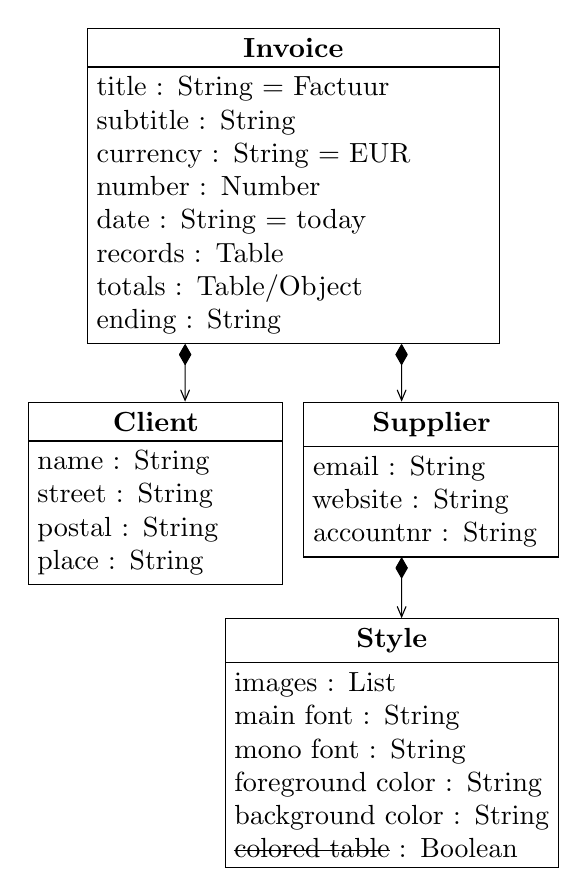
\begin{tikzpicture}
    \begin{class}[text width=5cm]{Invoice}{1.75,0}
        \attribute{title : String = Factuur}
        \attribute{subtitle : String}
        \attribute{currency : String = \cs{EUR}}
        \attribute{number : Number}
        \attribute{date : String = \cs{today}}
        \attribute{records : Table}
        \attribute{totals : Table/Object}
        \attribute{ending : String}
    \end{class}
    \begin{class}[text width=3cm]{Supplier}{3.5,-4.75}
        \attribute{email : String}
        \attribute{website : String}
        \attribute{accountnr : String}
    \end{class}
    \begin{class}[text width=3cm]{Client}{0,-4.75}
        \attribute{name : String}
        \attribute{street : String}
        \attribute{postal : String}
        \attribute{place : String}
    \end{class}
    \begin{class}[text width=4cm]{Style}{3,-7.5}
        \attribute{images : List}
        \attribute{main font : String}
        \attribute{mono font : String}
        \attribute{foreground color : String}
        \attribute{background color : String}
        \attribute{\sout{colored table} : Boolean}
    \end{class}
    \draw[umlcd style, diamond-angle 45] ($(Invoice.south west) - (-1.25,0)$) -- ($(Client.north) + (.375,0)$);
    \draw[umlcd style, diamond-angle 45] ($(Invoice.south east) + (-1.25,0)$) -- ($(Supplier.north) + (-.375,0)$);
    \draw[umlcd style, diamond-angle 45] ($(Supplier.south) + (-.375,0)$) -- ($(Style.north) + (.125,0)$);
\end{tikzpicture}

    \caption{Klassediagram Factuur}\label{fig:invoice-cd}
\end{figure}
Bij het opstellen van een factuur is het niet wenselijk om telkens alle klant- en leveranciersinformatie opnieuw in te voeren.
Daarom kunnen bepaalde aspecten van de factuurdata worden aangepast of weggelaten, afhankelijk van de gebruiksscenario's.

In de praktijk kunnen LaTeX-gebruikers bijvoorbeeld gebruikmaken van LaTeX-pakketten zoals \texttt{invoice}, \texttt{invoice2} of andere, die rekenkundige functionaliteiten bevatten zoals totaalbedragen en eindtotalen.

Bovendien kan de styling van de factuur, die momenteel op leveranciersniveau is geplaatst, direct onder het niveau van de leverancier worden geplaatst.
Dit komt omdat de styling in de praktijk waarschijnlijk niet zal verschillen, tenzij een leverancier meerdere afdelingen heeft die elk hun eigen specifieke kleuren of logo's vereisen.

Verder kunnen de titel en subtitel, die momenteel onder het niveau van de factuur zijn geplaatst, beter onder het niveau van de leverancier worden gehangen.
Dit komt omdat deze vaak alleen per leverancier verschillen en niet per factuur.

Een ander voorbeeld is het valutasymbool, dat momenteel op factuurniveau is geplaatst.
In de praktijk kan het echter handiger zijn om dit onder het niveau van de klant te plaatsen, aangezien het meestal alleen verschilt tussen verschillende klanten en niet per factuur voor dezelfde klant.

Ten slotte zijn alle styling gerelateerde oplossingen opgenomen in de factuurdata, zodat een gebruiker in de applicatie in staat is om dit aan te passen.
Voor LaTeX-gebruikers is dit echter niet nodig, omdat zij deze aanpassingen rechtstreeks in LaTeX zelf kunnen doen.

\subsection{Resultaat Voorbeeld}
Het project zelf bevat voorbeeldgegevens die resulteren in het volgende voorbeeld:
\begin{figure}[!ht]
    \centering
    \includegraphics[width=\linewidth]{ginvoice/ginvoice.pdf}
    \caption{Voorbeeldfactuur gegenereerd door GinVoice}
    \label{fig:voorbeeldfactuur}
\end{figure}
Het bovenstaande voorbeeld toont een gegenereerde factuur met behulp van de huidige implementatie van GinVoice.
Echter, op dit moment vereist het genereren van dit voorbeeld Python, wat voor template makers die hoofdzakelijk \LaTeX\ gebruiken, ongewenst is.
In het volgende hoofdstuk zullen we deze situatie aanpakken en laten zien hoe dit voorbeeld rechtstreeks kan worden gegenereerd met \LuaLaTeX.


    \section{YAML Interfaces with \texttt{lua-placeholders}}\label{sec:data}

This chapter demonstrates how YAML interfaces, also known as \textit{recipes}, can be used as interfaces for invoice templates and how they can be integrated into \LaTeX.
The ultimate goal is to provide an efficient and customizable invoicing interface that can be easily integrated into GinVoice.

\subsection{YAML Specifications}
Based on the data analysis in Chapter~\ref{sec:invoice data}, we can start working with the \textit{recipes}.
All \textit{recipes} are placed in the \texttt{recipes} directory relative to the \LaTeX\ project.
Alternatively, you can keep the same directory under \texttt{\$TEXMFHOME/tex/} to make the \textit{recipes} available everywhere.

\subsubsection{The Invoice}
The invoice recipe, \texttt{recipes/invoice.yaml}, specifies two relationships: \texttt{supplier} and \texttt{client}, as indicated in Chapter~\ref{sec:invoice data}.
\lstinputlisting[language=YAML,caption={\texttt{recipes/invoice.yaml}},linerange=1-5,numbers=left,xleftmargin=15pt]{demo/recipes/invoice.yaml}
How the corresponding recipes are loaded based on these values is described in Chapter~\ref{sec:preamble}.

The data within the invoice part can be standardized using a \texttt{default} field, as shown for \texttt{title}.
You can even invoke \LaTeX\ from a default value, including other parameters using \cs{param}.
\lstinputlisting[language=YAML,firstnumber=6,linerange=6-21,numbers=left,xleftmargin=15pt]{demo/recipes/invoice.yaml}
In addition to default values, temporary placeholders can also be specified.

The most complex part of the invoice is the invoice table.
Here, you can specify columns, just as you would for other data types.
\lstinputlisting[language=YAML,firstnumber=22,linerange=22-39,numbers=left,xleftmargin=15pt]{demo/recipes/invoice.yaml}
As mentioned earlier in Chapter~\ref{sec:invoice data}, for most \LaTeX\ users, the \texttt{total} column can be omitted and calculated using packages like \texttt{invoice2}.
Additionally, it would be necessary to make the \texttt{quantity} field of type \texttt{number} and add an extra field like \texttt{quantity type} to specify the correct notation for the \texttt{quantity} column.

For the grand totals, I have chosen the type \texttt{object} so that I can manually place the different totals in \LaTeX.
\lstinputlisting[language=YAML,firstnumber=40,linerange=40-51,numbers=left,xleftmargin=15pt]{demo/recipes/invoice.yaml}
The grand totals could also be handled in a more generic way, such as the \texttt{extra fields} field in the supplier recipe (see Chapter~\ref{sec:supplier spec}).

The last field of the invoice, \texttt{message}, uses a special YAML functionality, namely multiline strings in the default value.
\lstinputlisting[language=YAML,firstnumber=52,linerange=52-,numbers=left,xleftmargin=15pt]{demo/recipes/invoice.yaml}
By using the pipe (\texttt{|}), this mode is activated.
This construction is ideal for large texts, possibly with \LaTeX\ syntax.

\subsubsection{Client}
The client data does not have any special specifications compared to the invoice.
\lstinputlisting[language=YAML,caption={\texttt{recipes/client.yaml}},numbers=left,xleftmargin=15pt]{demo/recipes/client.yaml}
Alternatively, all address details could be specified as a \texttt{list} type, along with a specification, as seen in the \texttt{extra fields} for the supplier.
This would make the interface more generic but less adaptable within the \LaTeX\ context.

\subsubsection{Supplier}\label{sec:supplier spec}
In the case of the supplier recipe, the \texttt{style} field serves the same function as \texttt{supplier} and \texttt{client} in the invoice, allowing the user to choose which style to apply.
\lstinputlisting[language=YAML,caption={\texttt{recipes/supplier.yaml}},numbers=left,xleftmargin=15pt]{demo/recipes/supplier.yaml}

Another interesting field in this specification is \texttt{extra fields}.
This field uses the type \texttt{table} to allow additional information fields, such as the supplier's account number, VAT number, or other relevant details.
Using a table instead of a fixed number of fields gives the end user the flexibility to add as much extra information as needed without imposing limitations.

\subsubsection{Style}
In the style recipe, fonts, colors, and multiple images can be specified.
As mentioned earlier, for \LaTeX\ users, this could be completely omitted and specified directly in \LaTeX\ itself.
\lstinputlisting[language=YAML,caption={\texttt{recipes/style.yaml}},numbers=left,xleftmargin=15pt]{demo/recipes/style.yaml}
Noteworthy is the type for \texttt{images}, namely \texttt{list}.
In Chapter~\ref{sec:typesetting}, it is shown how this list is loaded at the bottom of the invoice.

\subsection{The New Invoice}
Now that the recipes are in order, we can move on to integrating them into \LaTeX.

\subsubsection{Loading Recipes in the Preamble}
The recipes are loaded using the macro \cs{loadrecipe}.
\lstinputlisting[language={[LaTeX]TeX},numbers=left,xleftmargin=15pt,firstnumber=44,linerange=44-47]{demo/invoice.tex}
For the \texttt{invoice} recipe, you can see that it receives the \meta{namespace} \cs{jobname}.
This is because the macro \cs{param} uses \cs{jobname} as the default \meta{name\-space}, simplifying its use.

The other recipes do not specify a \meta{namespace}, meaning they carry the base name of the path as the \meta{namespace}.
In this case, respectively \texttt{supplier}, \texttt{client}, and \texttt{style}.

\subsubsection{Currency}
Regarding the currency, I have chosen to disguise it in the \cs{currency} macro.
This is because it is also used in other files, such as \texttt{invoice.cls}.
\lstinputlisting[language={[LaTeX]TeX},numbers=left,xleftmargin=15pt,firstnumber=49,linerange=49]{demo/invoice.tex}
If the \meta{currency} is not set, the default value from \texttt{style.yaml} is used.
In this case, it defaults to \cs{EUR}.

\subsubsection{Loading Values}\label{sec:preamble}
I manage all YAML files related to the payload in corresponding directories.\\
\dirtree{%
    .1 \meta{project name}.
    .2 recipes.
    .3 \meta{recipe}.yaml.
    .2 invoices.
    .3 \meta{invoice-xxx}.yaml.
    .2 clients.
    .2 \textit{et cetera}.
}
\noindent
Values, also called the payload, are loaded similarly to recipes but with the macro \cs{loadpayload}.
Due to the relationships described in Chapter~\ref{sec:invoice data}, this is slightly more complex than recipes because \pkg{lua-placeholders} does not offer anything standard for this.
\lstinputlisting[language={[LaTeX]TeX},numbers=left,xleftmargin=15pt,firstnumber=51,linerange=51-54]{demo/invoice.tex}
For loading invoice values, it checks if a corresponding YAML file exists.
If so, that payload is loaded, and the experimental macro \cs{strictparams} is used, which will in the future result in errors when mandatory data is missing.

If no corresponding file is found, a default invoice template is compiled.

After loading the invoice data, we check if a client is specified in the invoice data.
We do this using \cs{hasparam}.
It concerns the invoice data, for which we do not need to specify a \meta{namespace}.
\lstinputlisting[language={[LaTeX]TeX},numbers=left,xleftmargin=15pt,firstnumber=56,linerange=56-58]{demo/invoice.tex}
Generally, \cs{param} is not intended for use within the preamble because it can also yield placeholders with \LaTeX\ formatting.
For such tricky situations, the \cs{rawparam} macro is written, as done for the client and supplier.
This macro has no optional arguments, which often causes problems with packages like \texttt{pgfkeys}.

\lstinputlisting[language={[LaTeX]TeX},numbers=left,xleftmargin=15pt,firstnumber=60,linerange=60-62]{demo/invoice.tex}
As seen, loading the supplier does not differ from loading the client.
However, there is still an additional action after loading the supplier, namely checking if the style can be loaded.
This is done in the same way as for the client and supplier themselves, but here you see that the \meta{namespace} must be set.
\lstinputlisting[language={[LaTeX]TeX},numbers=left,xleftmargin=15pt,firstnumber=64,linerange=64-72]{demo/invoice.tex}
For the style-related data, I have chosen to configure the values directly in the corresponding macros, such as \cs{setmainfont} and \cs{definecolor}, as long as a style is specified.
You could also choose to set the style values by default based on the default values specified in the style recipe, by placing the configuration outside the \cs{hasparam} block.

\subsection{Processing in Document}\label{sec:typesetting}
Before we can proceed to compile invoices, we have one task left, namely to set all values in the document itself.
\subsubsection{Header}
As mentioned earlier in Chapter~\ref{sec:legacy-invoice}, the \cs{makeheader} macro comes from \texttt{invoice.cls}.
For now, let's assume that \texttt{invoice.cls} has been modified so that it no longer causes errors and that \cs{makeheader} now expects the title and subtitle as arguments:
\lstinputlisting[language={[LaTeX]TeX},numbers=left,xleftmargin=15pt,firstnumber=76,linerange=76-79]{demo/invoice.tex}
In the example, there are only two differences compared to the old version, namely:\\
\cs{title}\hfill\textrightarrow\hfill\lstinline[language={[LaTeX]TeX}]|\param{title}|\\
\cs{subtitle}\hfill\textrightarrow\hfill\lstinline[language={[LaTeX]TeX}]|\param{subtitle}|\\
However, this time correctly passed to the \texttt{document\-class}.

\subsubsection{Information}
The left column of the information is quite tricky, as it contains both client information and invoice data such as number and date.
\lstinputlisting[language={[LaTeX]TeX},numbers=left,xleftmargin=15pt,firstnumber=80,linerange=80-91]{demo/invoice.tex}
You can see in the address lines that each line is terminated with a line break.
This could have also been achieved if, for example, there was a \texttt{address lines} field of type \texttt{list}.
Then, with \lstinline|\param[client]{address lines}|, that would have been solved in one go, given that \texttt{postal} and \texttt{place} are combined on one line in YAML\@.
The mentioned alternative assumes that the \cs{paramlistconjunction} macro is set to `\texttt{\textbackslash\textbackslash}', instead of the default value `\texttt{,\~}'.
\lstinputlisting[language={[LaTeX]TeX},numbers=left,xleftmargin=20pt,firstnumber=92,linerange=92-101]{demo/invoice.tex}
The right column of information is similar to the left, but it has an additional special field, namely \texttt{extra fields} of type \texttt{table}.
This allows adding a variable number of rows.
The same could potentially be applied to the client data in the left column.
Then it only remains to choose whether to place them above or below the invoice information.

\subsubsection{Table}
As mentioned earlier, standardizing the column definition is difficult.
On line 105, you can see what the \cs{columdefs} could have provided, except for the counters I used earlier.
\lstinputlisting[language={[LaTeX]TeX},numbers=left,xleftmargin=20pt,firstnumber=103,linerange=103-105]{demo/invoice.tex}
For the second argument of the \texttt{invoice} environment, a static header is set.
\lstinputlisting[language={[LaTeX]TeX},numbers=left,xleftmargin=20pt,firstnumber=106,linerange=106-107]{demo/invoice.tex}
For the third argument of the \texttt{invoice} environment, you can see how the grand totals are set in the table.
These totals are placed in the last two columns of each row, so that they align neatly with the rest of the table.
\lstinputlisting[language={[LaTeX]TeX},numbers=left,xleftmargin=20pt,firstnumber=108,linerange=108-113]{demo/invoice.tex}
In the final part of the table, you can see how each invoice item is set using \cs{formatrecords} and \cs{fortablerow}.
\lstinputlisting[language={[LaTeX]TeX},numbers=left,xleftmargin=20pt,firstnumber=114,linerange=114-119]{demo/invoice.tex}
The overall structure of the table still comes from the previous situation.
The notable difference compared to the new situation is that the data can be placed in all sorts of table structures since the data is decoupled from the \LaTeX\ and application domain, and the typesetting challenges are shifted to the \LaTeX\ domain.

\subsubsection{Closing Text and Images}
Where we previously saw an advanced YAML specification for the \texttt{message} field, the implementation within \LaTeX\ remains almost the same:
\lstinputlisting[language={[LaTeX]TeX},numbers=left,xleftmargin=20pt,firstnumber=121,linerange=121]{demo/invoice.tex}
The only difference is:\\
\cs{theending}\hfill\textrightarrow\hfill\lstinline|\param{message}|\\
However, for the images, it's a bit trickier to implement in \LaTeX\ due to the \texttt{list} type.
\lstinputlisting[language={[LaTeX]TeX},numbers=left,xleftmargin=20pt,firstnumber=122,linerange=122-]{demo/invoice.tex}
Where previously in Python, all images were neatly placed side by side, with a \cs{hspace} of \texttt{1.5em} between each image, I chose to apply half of that as \cs{hspace} on both sides of each image.
This is because the \cs{forlistitem} macro does not yet have a convenient way to do this, like \cs{param} does by setting \cs{paramlistconjunction} to `\lstinline|\hspace{1.5em}|'.


    \section{Execution}\label{sec:output}
% Advanced YAML payload examples, + sequence diagram command line
Now that the legacy invoice has been fully transformed, let's see what the result looks like.
% explain jobname

\subsection{The Template Version}
Without providing any values, we get the following result, as shown in Figure~\ref{fig:template}.\\
\setlength\fboxsep{0pt}%
\begin{figure}[!ht]%
    \fbox{\includegraphics[width=\linewidth-1pt]{invoice-template.pdf}}%
    \caption{\texttt{invoice-template.pdf}}\label{fig:template}%
\end{figure}
As mentioned earlier, \pkg{lua-placeholders} can only be compiled with \LuaLaTeX.
Additionally, the option \texttt{--shell-escape} is required to load YAML files.
The example can be compiled as follows:
\begin{lstlisting}[language=bash,caption={Compiling with \texttt{lualatex}}]
lualatex --shell-escape \
     --jobname=invoice-template \
     --output-directory=$(OUTPUT_DIR) \
     invoice
\end{lstlisting}
Where \texttt{\$(OUTPUT\_DIR)} is the desired output directory and \texttt{invoice-template} not corresponding to any of the payload files, therefore making it an invoice template.

However, if you are drafting a template, continually generating with \texttt{latexmk} is more user-friendly:
\begin{lstlisting}[language=bash,caption={Compiling with \texttt{latexmk}}]
latexmk -pvc -lualatex \
    --shell-escape \
    --jobname=invoice-template \
    --output-directory=$(OUTPUT_DIR) \
    invoice
\end{lstlisting}
This way, you don't have to recompile every time there's a change in \TeX, it happens automatically.
It's also very useful on the application level for previewing the result while filling in a form.

\subsection{YAML Values}
To get a filled-in invoice, we will need the following YAML files:

\dirtree{%
    .1 \meta{project dir}.
    .2 invoices.
    .3 \meta{invoice}.yaml.
    .2 suppliers.
    .3 \meta{supplier}.yaml.
    .2 styles.
    .3 \meta{style}.yaml.
    .2 clients.
    .3 \meta{client}.yaml.
}

This structure is based on the implementation described in Chapter~\ref{sec:preamble}.
Before discussing the contents of the YAML files, let's first consider alternative project structures.

\subsubsection{Alternative Project Structure}
Everyone is free to create their desired folder structure.
For example, you could place styles under\\
\hspace*{4em}\texttt{/suppliers/\meta{supplier}/style.yaml}\\
so that you can even omit the \texttt{style} field in the supplier recipe.
Another good example is placing the \texttt{clients} directory under the supplier level, so you don't accidentally mix clients of suppliers.
This could be achieved by doing the following:
\dirtree{%
    .1 \meta{project dir}.
    .2 suppliers.
    .3 \meta{supplier}.yaml.
    .3 \meta{supplier}.
    .4 \meta{client}.yaml.
}
\noindent
This way, the implementation for loading clients would require the variables \meta{supplier} and \meta{client}, and then proceed to the path\\
\hspace*{4em}\texttt{suppliers/\meta{supplier}/\meta{client}.yaml}.

The same consideration could be applied to the invoices, however, this is a more complex scenario, as the invoice data is based on the \cs{jobname} in the implementation of Chapter~\ref{sec:preamble}.
One possible solution for this is to manage the project per supplier.
You can then place the \textit{recipes} in the \texttt{\$TEXMFHOME/tex} directory so that they are present for all projects.
Here's an example of a possible project structure:\\
\begin{minipage}{.49\linewidth}
    \dirtree{%
        .1 \$HOME/texmf/tex.
        .2 recipes.
        .3 invoice.yaml.
        .3 client.yaml.
        .3 supplier.yaml.
        .3 style.yaml.
        .2 invoice.cls.
        .2 invoice.tex.
    }
\end{minipage}%
\hfill
\begin{minipage}{.49\linewidth}
    \dirtree{%
        .1 \meta{project dir}.
        .2 invoices.
        .3 \meta{invoice}.yaml.
        .2 clients.
        .3 \meta{client}.yaml.
        .2 supplier.yaml.
        .2 style.yaml.
    }
\end{minipage}
In this example, all data related to a supplier is separated, including the client information and the final invoices.

\subsection{Suppliers and Clients}\label{sec:supplier and client}
In the example result of GinVoice, a client named \textit{Juicing Joker} was shown.
In YAML, this would translate to:
\lstinputlisting[captionpos=b,caption={\texttt{clients/juicing-joker.yaml}}]{demo/clients/juicing-joker.yaml}

This way, the client can be referenced in the invoice with \texttt{juicing-joker}.

For the supplier, we saw \textit{Grapefruit Inc.}\ in the example, which translates to:
\lstinputlisting[captionpos=b,caption={\texttt{suppliers/grapefruit.yaml} or \texttt{grapefruit/supplier.yaml}}]{demo/suppliers/grapefruit.yaml}

\onecolumn
\begin{figure}[!ht]
%    \centering
    \begin{subfigure}{.32\linewidth}
        \fbox{\includegraphics[width=\linewidth-1pt]{invoice2-template.pdf}}
        \caption{\texttt{invoice-template.pdf}}\label{fig:result alt}
    \end{subfigure}\hfill
    \begin{subfigure}{.32\linewidth}
        \fbox{\includegraphics[width=\linewidth-1pt]{invoice-001.pdf}}
        \caption{\texttt{invoice-001.pdf}}\label{fig:result 1}
    \end{subfigure}\hfill
    \begin{subfigure}{.32\linewidth}
        \fbox{\includegraphics[width=\linewidth-1pt]{invoice-002.pdf}}
        \caption{\texttt{invoice-002.pdf}}\label{fig:result 2}
    \end{subfigure}
    \caption{Invoice Examples}\label{fig:pdfs}
\end{figure}
\begin{multicols}{2}
    And for the style:
    \lstinputlisting[captionpos=b,caption={\texttt{styles/grapefruit.yaml} or \texttt{grapefruit/style.yaml}}]{demo/styles/grapefruit.yaml}

    The advantage of the alternative project structure is that \texttt{invoice-template} automatically picks up the styling as well as the supplier information, as seen in Figure~\ref{fig:result alt}.

    \subsection{Invoices}
    To create an invoice that exactly matches the standard example of GinVoice, as shown in Figure~\ref{fig:result 1}, we use the following YAML example:
    \lstinputlisting[xleftmargin=15pt,numbers=left,linerange=-15,caption={\texttt{invoices/invoice-001.yaml}}]{demo/invoices/invoice-001.yaml}
    The actors \texttt{grapefruit} and \texttt{juicing-joker}, discussed in Chapter~\ref{sec:supplier and client}, are reflected in the invoice.
    With other values it could make the difference between figure~\ref{fig:result 1} and~\ref{fig:result 2}.
    Additionally, the example has the same general information to achieve the same result.
    In the \texttt{records} field, you can see that one row of the table takes up many lines.
    In the second row of the table, you can see that the \texttt{description} field has an empty value.
%    \columnbreak
    If the quotes are omitted in YAML, you'll get an error when converting to data.
    Since the rows don't differ too much from each other, we continue the example at the \texttt{totals} field:
    \lstinputlisting[xleftmargin=15pt,numbers=left,linerange=34-40,firstnumber=34]{demo/invoices/invoice-001.yaml}
%    The only difference between compiling the template version is the \cs{jobname}.
\end{multicols}
\twocolumn
\lstinputlisting[xleftmargin=15pt,numbers=left,linerange=41-,firstnumber=41]{demo/invoices/invoice-001.yaml}
Finally, in the example, we see the totals and the closing text.

This invoice can then be compiled with the following command:
\begin{lstlisting}[language=bash]
lualatex --shell-escape \
    --jobname=invoice-001 \
    --output-directory=$(OUTPUT_DIR) \
      invoice
\end{lstlisting}
Where both \texttt{invoice-001} and \texttt{invoice-002} correspond to actual YAML files.

%\begin{figure}[!ht]
%    \centering
%    \includegraphics[width=.8\linewidth]{invoice-002.pdf}%
%    \makebox[0pt][r]{%
%        \raisebox{-2em}{%
%            \colorbox{white}{\includegraphics[width=.8\linewidth]{invoice-001.pdf}}%
%        }\hspace*{1em}%
%    }%
%    \caption{Factuur 1 en 2}
%\end{figure}


    \section{Conclusie}\label{sec:conclusie}
In dit artikel hebben we niet alleen de implementatie van factuursjablonen in GinVoice onderzocht, maar ook een innovatieve methode voorgesteld om deze sjablonen naadloos te integreren met het \LaTeX-ecosysteem.
Door YAML te gebruiken als tussenlaag en \pkg{lua-placeholders} voor dynamische invoegingen, hebben we niet alleen een robuuste en flexibele oplossing geboden voor het genereren van facturen, maar ook een raamwerk gecreëerd waarin verschillende documentonderdelen, zoals klantinformatie, document-overkoepelend kunnen worden ingezet.

Deze aanpak biedt \LaTeX-gebruikers niet alleen de vrijheid om factuursjablonen naar wens aan te passen, maar opent ook de deur naar een breder scala aan toepassingen.
Door dezelfde YAML-gebaseerde structuur te gebruiken, kunnen verschillende documenten, zoals contracten en facturen, met gemak worden gegenereerd en onderhouden.
Dit vergroot niet alleen de consistentie tussen verschillende documenttypen, maar verhoogt ook de efficiëntie van het documentatieproces als geheel.

Het gebruik van \pkg{lua-placeholders} in combinatie met YAML maakt het mogelijk om dynamische content toe te voegen aan sjablonen, waardoor gebruikers een meer gestroomlijnde workflow ervaren.
Deze flexibiliteit maakt het gemakkelijk om gegevens en opmaak van verschillende documenten te scheiden, terwijl het tegelijkertijd de mogelijkheid biedt om deze onderdelen document-overkoepelend in te zetten.

Als conclusie biedt deze aanpak niet alleen een waardevolle bijdrage aan het optimaliseren van factureringsprocessen, maar opent het ook nieuwe mogelijkheden voor het efficiënt genereren en beheren van verschillende soorten documenten binnen een organisatie.


    \section{Discussion}

\subsection{\LaTeX\ Compilers}
In the article, I assume the \LuaLaTeX\ compiler.
For \LaTeX\ users using other compilers, \pkg{lua-placeholders} does not provide a solution.
Although some compilers still offer support for Lua, \pkg{lua-placeholders} does not take this into account.
Research and implementation could improve the adoption of \pkg{lua-placeholders} within the \LaTeX\ community.

\subsection{JSON vs YAML}
I did not delve into the choice of YAML over JSON in the article.
Both are intended for data, and while JSON is more well-known and has broader compatibility with programming languages, I chose YAML for the sake of readability of \LaTeX\ source code.
As demonstrated extensively, the files contain a lot of \LaTeX\ source code.
When using JSON, every backslash would need to be escaped.
For example:
\begin{lstlisting}[style=yaml,caption={YAML example}]
title: Invoice \param{number}
\end{lstlisting}
\begin{lstlisting}[style=json,caption={JSON example}]
{
    "title": "\\param{number}"
}
\end{lstlisting}
For a \LaTeX\ user, I find it more convenient to adjust values in YAML for testing purposes than in JSON.

\subsection{GinVoice Roadmap}
Development has been stagnant for some time, but I recently discovered that the solution can also work for Windows platforms.
Bringing GinVoice to the Windows platform significantly expands the target audience and, in my expectation, could garner more support for \LaTeX.

Regarding the introduction of \pkg{lua-placeholders}, there are still a few obstacles to overcome, such as challenges related to translation and the variable column definition, which is precisely a user-friendly part of the application that has not been discussed.


    \bibliographystyle{tugboat}%
    \bibliography{references}

    \makesignature
\end{document}
